\chapterimage{chap2.png} % Chapter heading image
\chapterspaceabove{5.75cm} % Whitespace from the top of the page to the chapter title on chapter pages
\chapterspacebelow{10cm} % Amount of vertical whitespace from the top margin to the start of the text on chapter pages
\chapter{Algorithm and Number}

Computer Science is most commonly known as an engineering subject, while the unanimous pursuit of all engineering subjects are solving problems. This chapter delves in to methods to solve problems, which is also known as \textbf{algorithm}. In the world of Computer Science, everything is proceeded in a methodical manner, and the very dependency of this is algorithm. Meanwhile, we will introduce pseudocode, one of the most important tools for algorithm analysis, as well as the representation of number in Computer Science.

%------------------------------------------------

\section{Numbers}
Every reader could be quite surprised when seeing the title for this section. Yes, numbers, we have known what is number since the very beginning when we get to learn math as toddlers. In this section, we will explain the system of number, not only will we figure out how numbers and their operations are defined, but how they are categorized.
\subsection{Typology of Numbers}
This part recalls the type of numbers we've learned since primary school and their set notations.
\label{sec:number}
\begin{enumerate}
  \item \textbf{Natural Numbers}
  \begin{itemize}
    \item Definition: Natural numbers are the set of positive integers used for counting and ordering, which do not include zero or negative numbers.
    \item Set Notation:
    \[
    \mathbb{N} = \{1, 2, 3, \ldots\}
    \]
  \end{itemize}

  \item \textbf{Integers}
  \begin{itemize}
    \item Definition: Integers are all the whole numbers including positive natural numbers, their negatives, and zero.
    \item Set Notation:
    \[
    \mathbb{Z} = \{\ldots, -3, -2, -1, 0, 1, 2, 3, \ldots\}
    \]
  \end{itemize}

  \item \textbf{Rational Numbers}
  \begin{itemize}
    \item Definition: Rational numbers are numbers that can be expressed as the quotient of two integers, a fraction \( \frac{a}{b} \), where \( a \) and \( b \) are integers and \( b \neq 0 \). The set includes all integers and fractions.
    \item Set Notation:
    \[
    \mathbb{Q} = \left\{\frac{a}{b} \mid a, b \in \mathbb{Z}, b \neq 0\right\}
    \]
  \end{itemize}

  \item \textbf{Irrational Numbers}
  \begin{itemize}
    \item Definition: Irrational numbers are real numbers that cannot be expressed as a ratio of two integers. The decimal expansion of irrational numbers is non-terminating and non-repeating. Examples include \(\pi\) and \(\sqrt{2}\).
    \item Set Notation:
    \[
    \mathbb{I} = \{x \in \mathbb{R} \mid x \notin \mathbb{Q}\}
    \]
    (Note: \(\mathbb{I}\) is used here for illustrative purposes and is not a standard symbol.)
  \end{itemize}

  \item \textbf{Real Numbers}
  \begin{itemize}
    \item Definition: The real numbers include both rational and irrational numbers, encompassing all points on an infinitely extended number line. The set of real numbers is continuous and is composed of all limits of sequences of rational numbers.
    \item Set Notation:
    \[
    \mathbb{R} = \{x \mid x \text{ is a limit of a sequence of rational numbers}\}
    \]
  \end{itemize}

  \item \textbf{Prime Numbers}
\begin{itemize}
  \item Definition: A prime number is a natural number greater than 1 that has no positive divisors other than 1 and itself. In other words, \( p \) is prime if \( p > 1 \) and if \( p \) is divisible only by 1 and \( p \).
  \item Set Notation:
  \[
  \mathbb{P} = \{p \in \mathbb{N} \mid p > 1 \text{ and } p \text{ has no divisors other than } 1 \text{ and } p\}
  \]
  \item Examples: The first few prime numbers are:
  \[
  2, 3, 5, 7, 11, 13, 17, \ldots
  \]
\end{itemize}
The following Venn diagram shows the relationship between different number sets.
\begin{figure}[H]
    \centering
    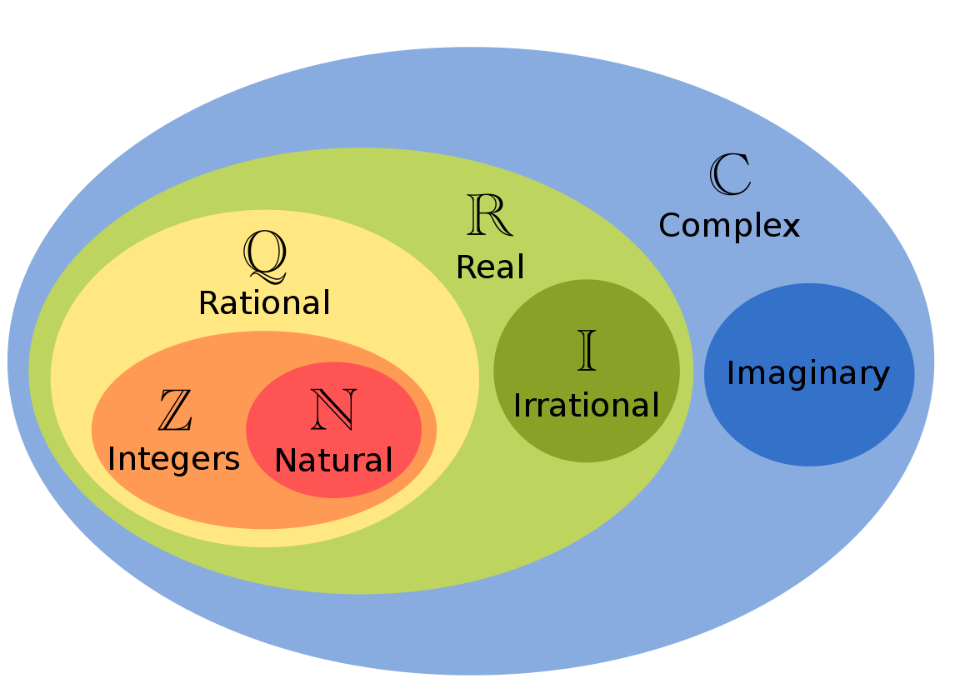
\includegraphics[width=0.5\linewidth]{venn.png}
    \caption{Venn Diagram of Number Sets}
    \label{venn}
\end{figure}

\begin{remark}
    Complex number is currently not a something necessary, as our discussion so far only falls in the real number set.
\end{remark}

\subsection{The Real Number System}
Considering the real numbers are the only system involved so far this book, here, we provide a new mathematical perspective that is different what we were taught, to understand the real number system. We will introduce three axioms that real number holds.
\begin{definition}[Field Axioms]\label{axi:field}
A set \( S \) with operations \( + \) and \( \cdot \) and distinguished elements 0 and 1 with \( 0 \neq 1 \) is a \emph{field} if the following properties hold for all \( x, y, z \in S \):

\begin{itemize}
  \item[A0:] \( x + y \in S \) \hfill Closure
  \item[A1:] \( (x + y) + z = x + (y + z) \) \hfill Associativity
  \item[A2:] \( x + y = y + x \) \hfill Commutativity
  \item[A3:] \( x + 0 = x \) \hfill Identity
  \item[A4:] given \( x \), there is a \( w \in S \) such that \( x + w = 0 \) \hfill Inverse
  \item[M0:] \( x \cdot y \in S \) \hfill Closure
  \item[M1:] \( (x \cdot y) \cdot z = x \cdot (y \cdot z) \) \hfill Associativity
  \item[M2:] \( x \cdot y = y \cdot x \) \hfill Commutativity
  \item[M3:] \( x \cdot 1 = x \) \hfill Identity
  \item[M4:] for \( x \neq 0 \), there is a \( w \in S \) such that \( x \cdot w = 1 \) \hfill Inverse
  \item[DL:] \( x \cdot (y + z) = x \cdot y + x \cdot z \) \hfill Distributive Law
\end{itemize}

\end{definition}
The operations \( + \) and \( \cdot \) are called addition and multiplication. The elements 0 and 1 are the additive identity element and the multiplicative identity element, respectively.   


It follows from these axioms that the additive inverse and multiplicative inverse (of a nonzero \( x \)) are unique. The additive inverse of \( x \) is the \textbf{negative} of \( x \), written as \( -x \). To define subtraction of \( y \) from \( x \), we let \( x - y = x + (-y) \). The multiplicative inverse of \( x \) is the \textbf{reciprocal} of \( x \), written as \( x^{-1} \). \textbf{The element 0 has no reciprocal}. To define division of \( x \) by \( y \) when \( y \neq 0 \), we let \( \frac{x}{y} = x \cdot (y^{-1}) \). We write \( x \cdot y \) as \( xy \) and \( x \cdot x \) as \( x^2 \). We use parentheses where helpful to clarify the order of operations.

\begin{definition}[Order Axioms]\label{axi:order}
     A positive set in a field \( F \) is a set \( P \subset F \) such that for \( x, y \in F \),

\begin{itemize}
  \item[P1:] \( x, y \in P \) implies \( x + y \in P \) \hfill Closure under Addition
  \item[P2:] \( x, y \in P \) implies \( xy \in P \) \hfill Closure under Multiplication
  \item[P3:] \( x \in F \) implies exactly one of \( x = 0 \), \( x \in P \), \( -x \in P \) \hfill Trichotomy
\end{itemize}

An ordered field is a field with a positive set \( P \). In an ordered field, we define \( x < y \) to mean \( y - x \in P \). The relations \( \leq, >, \) and \( \geq \) have analogous definitions in terms of \( P \).

Note that \( P = \{ x \in F : x > 0\} \). Another phrasing of trichotomy is that each ordered pair \( (x, y) \) satisfies exactly one of \( x < y \), \( x = y \), \( x > y \).
If \( S \subseteq F \), then \( \beta \in F \) is an \textbf{upper bound} for \( S \) if \( x \leq \beta \) for all \( x \in S \).
\end{definition}
\begin{definition}[Completeness Theorem]
     An ordered field \( F \) is complete if every nonempty subset of \( F \) that has an upper bound in \( F \) has a least upper bound in \( F \).
\end{definition}

    This theorem ensures the square roots of positive real numbers.

\end{enumerate}

Axiom \autoref{axi:field} and \autoref{axi:order} imply many familiar property of arithmetic:

\begin{proposition}[Arithmetic in $\mathbb{N}$, $\mathbb{Z}$, $\mathbb{Q}$]
Each of $\mathbb{N}$, $\mathbb{Z}$, and $\mathbb{Q}$ is closed under addition and multiplication, $\mathbb{Z}$ and $\mathbb{Q}$ are closed under subtraction, and the set of nonzero numbers in $\mathbb{Q}$ is closed under division.
\end{proposition}

The next four propositions state properties of an ordered field $F$. All statements apply for each choice of $x, y, z, u, v \in F$.

\begin{proposition}
Elementary consequences of the field axioms.
\begin{align*}
    \text{a)} &\quad x + z = y + z \text{ implies } x = y \\
    \text{b)} &\quad x \cdot 0 = 0 \\
    \text{c)} &\quad (-x)y = -(xy) \\
    \text{d)} &\quad -x = (-1)x \\
    \text{e)} &\quad (-x)(-y) = xy \\
    \text{f)} &\quad xz = yz \text{ and } z \neq 0 \text{ imply } x = y \\
    \text{g)} &\quad xy = 0 \text{ implies } x = 0 \text{ or } y = 0
\end{align*}
\end{proposition}

\begin{proposition}[Properties of an ordered field.]
\begin{align*}
    \text{O1:} &\quad x \leq x && \text{Reflexive Property} \\
    \text{O2:} &\quad x < y \text{ and } y < x \text{ imply } x = y && \text{Antisymmetric Property} \\
    \text{O3:} &\quad x < y \text{ and } y < z \text{ imply } x < z && \text{Transitive Property} \\
    \text{O4:} &\quad \text{At least one of } x < y \text{ and } y < x \text{ holds} && \text{Total Ordering Property}
\end{align*}
\end{proposition}

\begin{proposition}[More properties of an ordered field.]
\begin{align*}
    \text{F1:} &\quad x \leq y \text{ implies } x + z \leq y + z && \text{Additive Order Law} \\
    \text{F2:} &\quad x < y \text{ and } 0 < z \text{ imply } xz < yz && \text{Multiplicative Order Law} \\
    \text{F3:} &\quad x < y \text{ and } w < v \text{ imply } x + w < y + v && \text{Addition of Inequalities} \\
    \text{F4:} &\quad 0 \leq x \text{ and } 0 \leq w \text{ imply } xw \leq xw && \text{Multiplication of Inequalities}
\end{align*}
\end{proposition}

\begin{proposition}[Still more properties of an ordered field.]
\begin{align*}
    \text{(a)} &\quad x < y \text{ implies } -y < -x \\
    \text{(b)} &\quad x \leq y \text{ and } z \leq 0 \text{ imply } yz \leq xz \\
    \text{(c)} &\quad 0 \leq x \text{ and } 0 \leq y \text{ imply } 0 \leq xy \\
    \text{(d)} &\quad 0 \leq x^2 \\
    \text{(e)} &\quad 0 < 1 \\
    \text{(f)} &\quad 0 < x \text{ implies } 0 < x^{-1} \\
    \text{(g)} &\quad 0 < x < y \text{ implies } 0 < y^{-1} < x^{-1}
\end{align*}
\end{proposition}

\subsection{Floor, Ceiling, and Remainder}
This Section discusses more form numbers that may not be as familiar as real numbers. We first introduce 
\textbf{Integer Function}:
\begin{definition}[Floor and Ceiling]
    If \( x \) is any real number, we write
\[
\lfloor x \rfloor = \text{the greatest integer less than or equal to \( x \) (the floor of \( x \))}
\]
\[
\lceil x \rceil = \text{the least integer greater than or equal to \( x \) (the ceiling of \( x \))}
\]
\end{definition}
Note that the $x$ could be not just a variable, but a mathematical expression.
\begin{example}
    \[
\lfloor \sqrt{2} \rfloor = 1, \quad \lceil \sqrt{2} \rceil = 2, \quad \left\lceil \frac{1}{2} \right\rceil = 0, \quad \left\lfloor -\frac{1}{2} \right\rfloor = 0, \quad \left\lceil -\frac{1}{2} \right\rceil = -1 \ (\text{not zero!});
\]
\end{example}

\subsubsection{Properties of Integer Function}
We will look into the properties of integer function with its graph. 
    \begin{figure}[H]
        \centering
        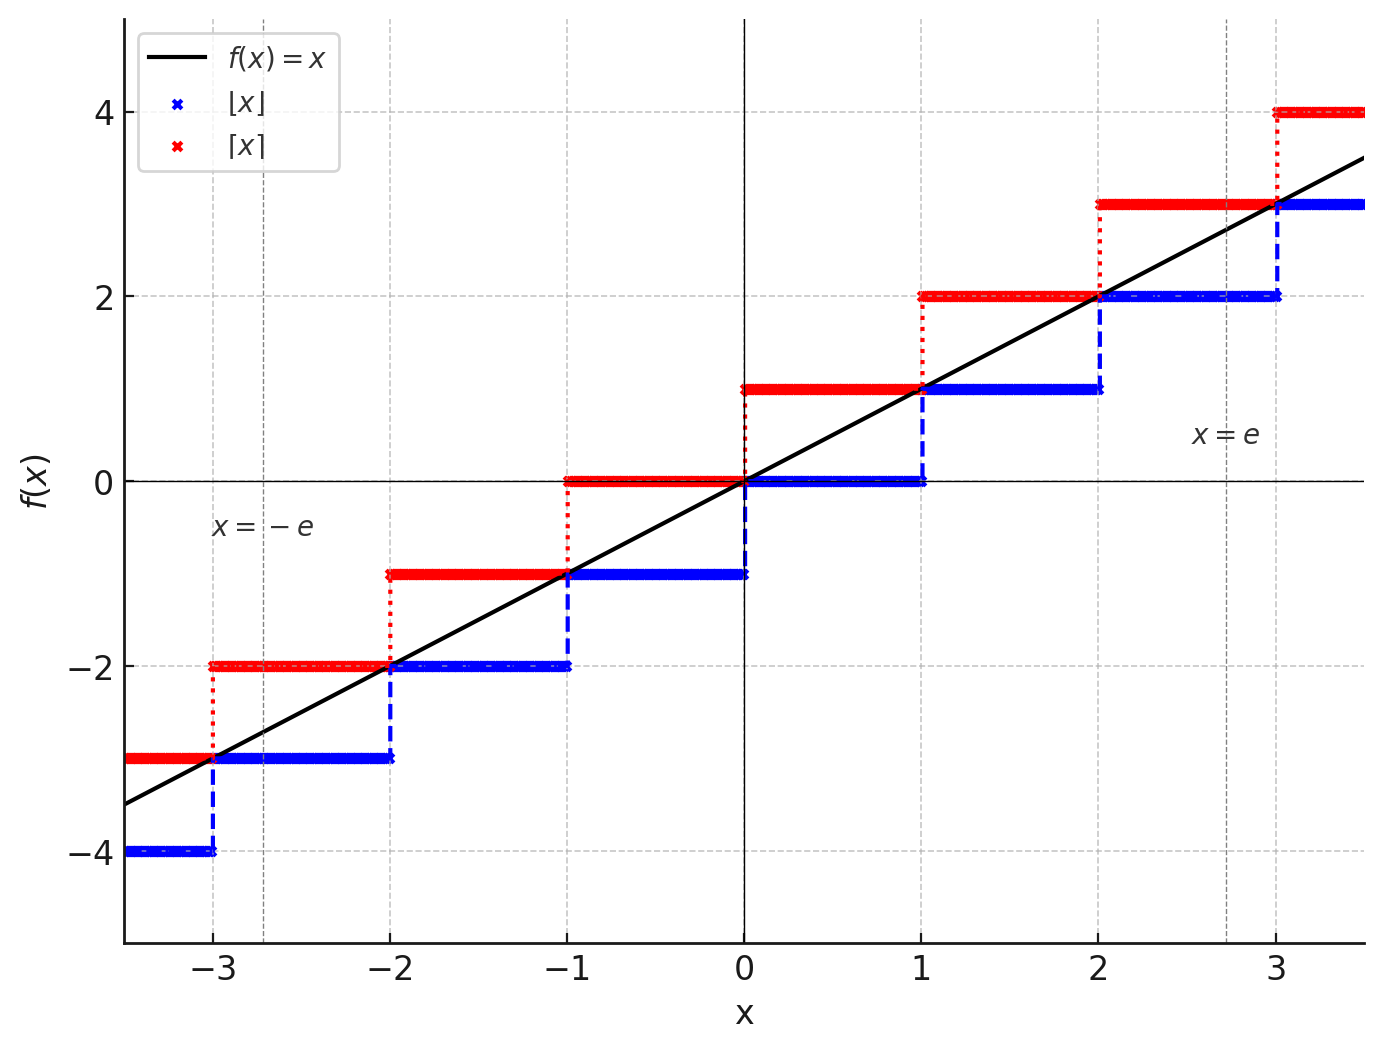
\includegraphics[width = 0.75\linewidth]{intfunc.png}
        \caption{Visualization of $\lceil x \rceil \text{ and } \lfloor x \rfloor$}
    \end{figure}

\begin{theorem}[Properties of Integer Function]
    Keep in mind the following important properties of integer function, which is 
    often used in algorithm analysis or other mathematical proof.
    \begin{enumerate}
        \item $\lfloor x \rfloor \leq x \leq \lceil x \rceil$
        \item  $\forall x\in \mathbb{Z} \text{, } \lceil x \rceil = \lfloor x \rfloor$
        \item $x \notin \mathbb{Z} \iff  \lceil x \rceil =  \lfloor x \rfloor+ 1  $
        \item $\lfloor -x \rfloor = -\lceil x \rceil $; $\lceil-x \rceil = - \lfloor x \rfloor$
        \item $x - 1 < \lfloor x \rfloor \leq x \leq \lceil x \rceil < x + 1$
    \end{enumerate}
\end{theorem}
The proofs to these conclusions are quite basic, and is therefore not provided here.

\subsubsection{Remainder and Integer Function}
We introduce a new operation that we have learned before in this section with its notation.
\begin{notation}[modulo operator]
    The modulo operation, denoted as \( a \bmod n \), finds the remainder when one integer \( a \) is divided by another integer \( n \). 
    If \( a \) divided by \( n \) gives a quotient \( q \) with remainder \( r \), then \( a = nq + r \), and \( r \) would be the result of \( a \bmod n \).
\end{notation}

Moving back to the integer function, we have:
\begin{theorem}
    $$\forall x, y \in \mathbb{R}, x \bmod y = x - y\left\lfloor \frac{x}{y} \right\rfloor, \quad \text{if } y \neq 0; \quad x \bmod 0 = x$$
\end{theorem}
Below is the proof to the first conclusion, where the properties of integer function are applied.
\begin{proof}
    By the Division Algorithm, for any integer \( x \) and any positive integer \( y \), there exist unique integers \( q \) and \( r \) such that \( x = qy + r \) and \( 0 \leq r < |y| \), where \( q \) is the quotient and \( r \) is the remainder. The floor function \( \left\lfloor \frac{x}{y} \right\rfloor \) yields the largest integer less than or equal to \( \frac{x}{y} \), which by definition is the quotient \( q \). Thus, we have:
\[
\left\lfloor \frac{x}{y} \right\rfloor = q
\]
and therefore:
\[
y\left\lfloor \frac{x}{y} \right\rfloor = yq
\]
Subtracting this from \( x \) gives:
\[
x - y\left\lfloor \frac{x}{y} \right\rfloor = x - yq = r
\]
The uniqueness of the quotient and remainder in the Division Algorithm ensures that this value of \( r \) is the remainder from the modulus operation. Therefore, we have:
\[
x \mod y = x - y\left\lfloor \frac{x}{y} \right\rfloor
\]
which is the remainder when \( x \) is divided by \( y \), completing the proof.

\end{proof}
Also, from definition, by dividing $y$ on both sides of the equation:
$$0\leq \frac{x}{y} - \lfloor\frac{x}{y}\rfloor = \frac{x \bmod y}{y} < 1$$
Among which, $x \bmod y <y$. 
\begin{proof}
    
        By the definition of the modulo operation, \( x \mod y \) can be written as \( x - y\left\lfloor \frac{x}{y} \right\rfloor \). Since \( \left\lfloor \frac{x}{y} \right\rfloor \) is the greatest integer less than or equal to \( \frac{x}{y} \), we have:
        \[
        x - y\left\lfloor \frac{x}{y} \right\rfloor \geq x - y \cdot \frac{x}{y} = x - x = 0.
        \]
        Furthermore, because \( \left \lfloor \frac{x}{y} \right\rfloor \) is less than \( \frac{x}{y} \), it follows that:
        \[
        x - y\left\lfloor \frac{x}{y} \right\rfloor < x - y \cdot \left(\frac{x}{y} - 1\right) = y.
        \]
        Hence, \( 0 \leq x \mod y < y \).

\end{proof}
And we have:
\begin{corollary}
    By above-mentioned conclusions:
    \begin{itemize}
        \item[a)] If $y > 0, \text{ then } 0 \leq x \bmod y < y$.
        \item[b)] If $y < 0, \text{ then}  0 \geq x \bmod y > y$.
        \item[c)]  $x - (x \bmod y) \text{ is an integral multiple of } y$.
    \end{itemize}
\end{corollary}
We call $x \bmod y$ the remainder when $x$ is divided by $y$. We call $\lfloor \frac{x}{y} \rfloor$ the quotient.
We have \( x \bmod y = 0 \) if and only if \( x \) is a multiple of \( y \), that is, if and only if \( x \) is divisible by \( y \). The notation \( y \mid x \), read ``\( y \) divides \( x \)'', means that \( y \) is a positive integer and \( x \bmod y = 0 \).
\subsection{exercises}
\begin{exercise}
    
        Let \( F \) be a field consisting of exactly three elements \( 0, 1, x \). Prove that \( x + x = 1 \) and that \( x \cdot x = 1 \). Obtain the addition and multiplication tables for \( F \).
        
\end{exercise}
    Hint: Think on the property of filed: inverse of addition and multiplication.
    \begin{proof}
        Since \( F \) is a field, it has the properties of both a group under addition and a group under multiplication (excluding \( 0 \) for the latter).
        
        \textbf{Part 1: Proof that \( x + x = 1 \)}
        \begin{enumerate}
            \item In a group, every element has an additive inverse. In \( F \), the additive inverse of \( 0 \) is \( 0 \) itself, since \( 0 + 0 = 0 \).
            \item The additive inverse of \( 1 \) cannot be \( 1 \) itself because \( 1 + 1 = 1 \) would imply \( 1 = 0 \), which is a contradiction. Therefore, \( 1 \)'s additive inverse must be some other element of \( F \), which can only be \( x \). Hence, \( 1 + x = 0 \).
            \item The element \( x \) must also have an additive inverse in \( F \), which cannot be \( 0 \) (as \( 0 \)'s inverse is \( 0 \)) and cannot be \( 1 \) (as \( 1 \)'s inverse is \( x \)). The only option left is \( x \) itself. Thus, \( x + x = 0 \).
            \item Given \( x + x = 0 \) and \( 1 + x = 0 \), by the cancellation law, it must be that \( x = 1 \). However, this contradicts the assumption that \( x \) is distinct from \( 1 \). Therefore, our assumption that \( x + x = 0 \) is incorrect.
            \item The only remaining possibility is \( x + x = 1 \).
        \end{enumerate}
        
        \textbf{Part 2: Proof that \( x \cdot x = 1 \)}
        \begin{enumerate}
            \item Similarly, in a multiplicative group (excluding \( 0 \)), every non-zero element has a multiplicative inverse. For \( 1 \), the multiplicative inverse is \( 1 \) itself since \( 1 \cdot 1 = 1 \).
            \item The element \( x \) must have a multiplicative inverse. It cannot be \( 0 \) since \( 0 \) is not invertible, and it cannot be \( 1 \) since \( 1 \) is already serving as its own inverse.
            \item The only remaining option for the multiplicative inverse of \( x \) is \( x \) itself. Hence, \( x \cdot x = 1 \).
        \end{enumerate}

        Now we construct the addition and multiplication tables for \( F \):

        \noindent
        \begin{minipage}{.5\textwidth}
        \centering
        \textbf{Addition Table:}
        \[
        \begin{array}{c|ccc}
        + & 0 & 1 & x \\
        \hline
        0 & 0 & 1 & x \\
        1 & 1 & x & 0 \\
        x & x & 0 & 1 \\
        \end{array}
        \]
        \end{minipage}%
        \begin{minipage}{.5\textwidth}
        \centering
        \textbf{Multiplication Table:}
        \[
        \begin{array}{c|ccc}
        \times & 0 & 1 & x \\
        \hline
        0 & 0 & 0 & 0 \\
        1 & 0 & 1 & x \\
        x & 0 & x & 1 \\
        \end{array}
        \]
        \end{minipage}
        \end{proof}
\begin{problem}
    Is there a field with exactly four elements? Is there a field with exactly six elements?
\end{problem}


\begin{exercise}
    Let \( n \) be an integer, and let \( x \) be a real number. Prove that:
\begin{enumerate}
    \item[a)] \( \lfloor x \rfloor < n \) if and only if \( x < n \);
    \item[b)] \( n \leq \lfloor x \rfloor \) if and only if \( n \leq x \);
    \item[c)] \( \lfloor x \rfloor \leq n \) if and only if \( x \leq n \);
    \item[d)] \( n < \lfloor x \rfloor \) if and only if \( n < x \);
    \item[e)] \( \lfloor x \rfloor = n \) if and only if \( x - 1 < n \leq x \) and if and only if \( n \leq x < n + 1 \);
    \item[f)] \( \lfloor x \rfloor = n \) if and only if \( x \leq n < x + 1 \) and if and only if \( n - 1 < x \leq n \).
\end{enumerate}
\end{exercise}
\begin{proof}
    \textbf{Part (a):} By definition, \( \lfloor x \rfloor \) is the greatest integer less than or equal to \( x \). Therefore, \( \lfloor x \rfloor < n \) means that \( x \) is less than \( n \) but not equal to it since \( \lfloor x \rfloor \) cannot be greater than \( x \).
    
    \textbf{Part (b):} If \( n \leq \lfloor x \rfloor \), then \( n \) must also be less than or equal to \( x \) because \( \lfloor x \rfloor \) is the greatest integer less than or equal to \( x \).
    
    \textbf{Part (c):} The statement \( \lfloor x \rfloor \leq n \) indicates that the largest integer less than or equal to \( x \) is also less than or equal to \( n \), which directly implies \( x \leq n \).
    
    \textbf{Part (d):} If \( n < \lfloor x \rfloor \), then \( n \) is strictly less than the integer part of \( x \), which means that \( n \) is also strictly less than \( x \).
    
    \textbf{Part (e):} For \( \lfloor x \rfloor = n \) to be true, \( x \) must be greater than \( n - 1 \) but not reach \( n + 1 \), hence the inequality \( x - 1 < n \leq x \) and \( n \leq x < n + 1 \).
    
    \textbf{Part (f):} Similarly, \( \lfloor x \rfloor = n \) if \( x \) has not reached \( n + 1 \) yet, which is the same as saying \( x \leq n < x + 1 \), and also if \( x \) is greater than \( n - 1 \) and less than or equal to \( n \), hence \( n - 1 < x \leq n \).
    \end{proof}

        \begin{exercise}
            Using the previous exercise, prove that \( \lfloor -x \rfloor = -\lceil x \rceil \).
            \end{exercise}
            
            \begin{proof}
                From the previous exercise, we have the following properties of the floor function for a real number \( x \) and an integer \( n \):
                \begin{enumerate}
                    \item \( x - 1 < \lfloor x \rfloor \leq x \);
                    \item \( n \leq x \) if and only if \( n \leq \lfloor x \rfloor \).
                \end{enumerate}
                Using these properties, we want to show that \( \lfloor -x \rfloor = -\lceil x \rceil \).
                
                Consider the number \( -x \). Applying property 1, we get:
                \[ -x - 1 < \lfloor -x \rfloor \leq -x \]
                Adding 1 to all parts of the inequality, we obtain:
                \[ -x < \lfloor -x \rfloor + 1 \leq -x + 1 \]
                Since \( \lceil x \rceil \) is the smallest integer greater than or equal to \( x \), \( \lfloor -x \rfloor + 1 \) is the smallest integer greater than \( -x \), which is \( -\lfloor x \rfloor \). Thus:
                \[ \lfloor -x \rfloor = -\lfloor x \rfloor - 1 = -\lceil x \rceil \]
                This completes the proof.
            \end{proof}

    \begin{exercise}
        Prove that $\displaystyle \lceil ( k-1) /2\rceil =\lfloor k/2\rfloor \ $and $\displaystyle \lfloor ( k-1) /2\rfloor =\lceil k/2\rceil \ $ $\displaystyle \forall \ k\ \in \mathbb{Z} .$
    \end{exercise}
    \begin{proof}
        We will prove the statement by cases.

        When $k$ is even, let $k=2n$. $\lceil (2n-1)/2\rceil = \lceil n - \frac{1}{2}\rceil=n, and \lfloor 2n/2\rfloor = n$.

        When $k$ is odd, let $k=2n+1$. $\lceil 2n/2 \rceil = n$, and $\lfloor2n+1/2\rfloor=\lfloor n+\frac{1}{2}=n$.
        
        The proof for $\displaystyle \lfloor ( k-1) /2\rfloor =\lceil k/2\rceil$ is similar.
    \end{proof}
%------------------------------------------------------------






\section{Algorithm and Algorithm Analysis}
	This Section discusses what is algorithm, and more importantly, how algorithms
	are assessed.

    \subsection{Algorithm}
    \subsubsection{What is an Algorithm?}
    \begin{definition}[Algorithm] \label{def:algo}
        An algorithm is a well-defined, step-by-step procedure or sequence of instructions designed to solve a specific class of problems:
        \begin{itemize}
            \item Each step in an algorithm must be clear and unambiguous. 
            \item Algorithms must be solvable, meaning they should be able to produce a correct solution for any valid input within a finite amount of time.
            \item An algorithm must terminate, i.e., it should have a defined end, at which point the goal has been achieved and the final output is produced.
        \end{itemize} 
    \end{definition}
    Here is an example of multiplication algorithm for better understanding of the concept.
    \begin{example}[Russian Peasant Multiplication]
        To find the product of integers \( M \) and \( N \), both larger than one:

        \begin{enumerate}
            \item Start two columns on a page, one labeled ``A'' and the other ``B''; and put the value of \( M \) under A and the value of \( N \) under B.
            
            \item Repeat
            \begin{itemize}
                \item[(a)] calculate a new A-value by multiplying the old A-value by 2; and
                \item[(b)] calculate a new B-value by dividing the old B-value by 2 and reducing the result by a half if necessary to obtain an integer;
            \end{itemize}
            Until the B-value equals one.
            
            \item Go down the columns crossing out the A-value whenever the B-value is even.
            
            \item Add up the remaining A-values and ``return'' the sum.
        \end{enumerate}
    \end{example}
    To show how it works, assume $A=73$ and $B=41$.

\begin{table}[H]
\centering
\begin{tabular}{c|c}
\hline
A & B \\
\hline
73 & 41 \\
146 & 20 (20\(\frac{1}{2}\) is reduced to 20) \\
292 & 10 \\
584 & 5 \\
1168 & 2 (2\(\frac{1}{2}\) is reduced to 2) \\
2336 & 1 \\
\hline
\end{tabular}
\caption{Execution of RPM}
\end{table}

Sum of the remaining A-values: $2336+584+73=2993$.

Let's review this algorithm referring to definition \autoref{def:algo}. 
\begin{enumerate}
    \item Clarity and Accuracy: All the instructions are clear and manipulable, nothing is ambiguous.
    
    \item Solvability: It is no doubt that for any two real numbers, we can find their product.
    
    \item Termination: For which ever numbers, we can always solve the problem in limited steps, as the terminate condition is when $B=1$, while B is divided by 2 (integer division) repetitively. 
\end{enumerate}

Hence, the RPM is a good example of algorithm, and with this, we could tell whether
something else is an algorithm or not.
\subsubsection{Pseudocode}
Pseudocode is a simplified, half-code, half-natural language script used by software developers and algorithm designers to outline the structure of a program or algorithm. It's not executable code, but rather a high-level representation of the algorithm's logic. The purpose of pseudo-code is to express the design of an algorithm in a form that can be easily translated into actual programming languages. It is written in a way that is understandable to people who do not necessarily know the syntax of programming languages. Pseudo-code allows the designer to focus on the core logic of the algorithm without getting bogged down with the syntactic details of a particular programming language. It often uses control structures like if-then-else, while, for, and others that are common to many high-level languages.
Understanding pseudocode is quite easy as it quite close to natural languages.

Here's the RPM transcribed in pseudocode:
\begin{algorithm}[H]
	\caption{Russian Peasant Multiplication}\label{alg:rpm}
	\begin{algorithmic}[1]
	\Procedure{RPM}{$A, B$}
		\State $product \gets 0$
		\While{$B > 0$}
			\If{$B$ is odd}
				\State $product \gets product + A$
			\EndIf
			\State $A \gets A \times 2$
			\State $B \gets B \div 2$
		\EndWhile
		\State \textbf{return} $product$
	\EndProcedure
	\end{algorithmic}
	\end{algorithm}

    To explicit:
    \begin{itemize}
        \item \textbf{procedure RPM(A, B)}: Defines a procedure or function named `RPM` taking two parameters `A` and `B`.
        \item \textbf{product $\leftarrow$ 0}: The assignment operator `$\leftarrow$` is used to assign the value on the right (0 here) to the variable on the left (`product`).
        \item \textbf{while B $>$ 0 do}: Begins a `while` loop that continues as long as the condition `B $>$ 0` is true. The `do` indicates that the following block of code will execute if the condition is met.
        \item \textbf{if B is odd then}: A conditional statement that checks if `B` is odd. If it is, the subsequent statement is executed.
        \item \textbf{product $\leftarrow$ product + A}: An assignment operation that adds `A` to `product` and assigns the sum back to `product`.
        \item \textbf{end if}: Marks the end of the `if` statement.
        \item \textbf{A $\leftarrow$ A $\times$ 2}: Multiplies the value of `A` by 2 and then assigns the result back to `A`.
        \item \textbf{B $\leftarrow$ B $\div$ 2}: Divides the value of `B` by 2 (integer division) and assigns the result back to `B`.
        \item \textbf{end while}: Marks the end of the `while` loop.
        \item \textbf{return product}: The `return` statement indicates the output or result of the procedure, which here is the value of the variable `product`.
        \item \textbf{end procedure}: Marks the end of the `RPM` procedure.
    \end{itemize}
	All later algorithms in this book will be presented using pseudocode.
%------------------------------------------------

\subsection{Algorithm Analysis}

\par Now let's take a look at this algorithm from another aspects. Is this a good or a bad algorithm. People assess algorithms by examine its \textbf{complexity}, which could be either \textbf{space complexity} or \textbf{time complexity}. The former refers to the the relationship between the input and the space needed to execute the algorithm, the latter, similarly, refers to the time needed. Many tools are available to quantify complexity, for both space and time complexity, \textbf{the big O notation} is the most common measurement. 
\begin{definition}[The Big O Notation]\label{Big O}
    Big O notation is used to classify algorithms according to how their running time or space requirements grow as the input size grows. The notation describes an upper limit on the time an algorithm could possibly take to complete, given the size of the input. For a function \( f(n) \), where n is the scale of input for the algorithm, the Big O notation is formally defined as follows with $c$ as a positive constant:
    $$O(f(n)) = \{ g(n) : \text{Where } c \text{ and } n_0 
	\text{ such that } 0 \leq g(n) \leq c \cdot f(n) \text{ for all } n \geq n_0 \}$$
\end{definition}

The following table provides common time complexities using Big O notation:

\begin{table}[ht]
\centering
\begin{tabular}{@{}cc@{}}
\toprule
\( f(n) \) & Description \\ \midrule
1 & Constant \\
\( \log n \) & Logarithmic \\
n & Linear \\
\( n \log n \) & Linearithmic \\
\( n^2 \) & Quadratic \\
\( n^3 \) & Cubic \\
\( 2^n \) & Exponential \\ 
\(n!\) & Factorial \\
\bottomrule
\end{tabular}
\caption{Common time complexities in Big O notation}
\end{table}
We can visualize it using function graph
\begin{figure}[H]
    \centering
    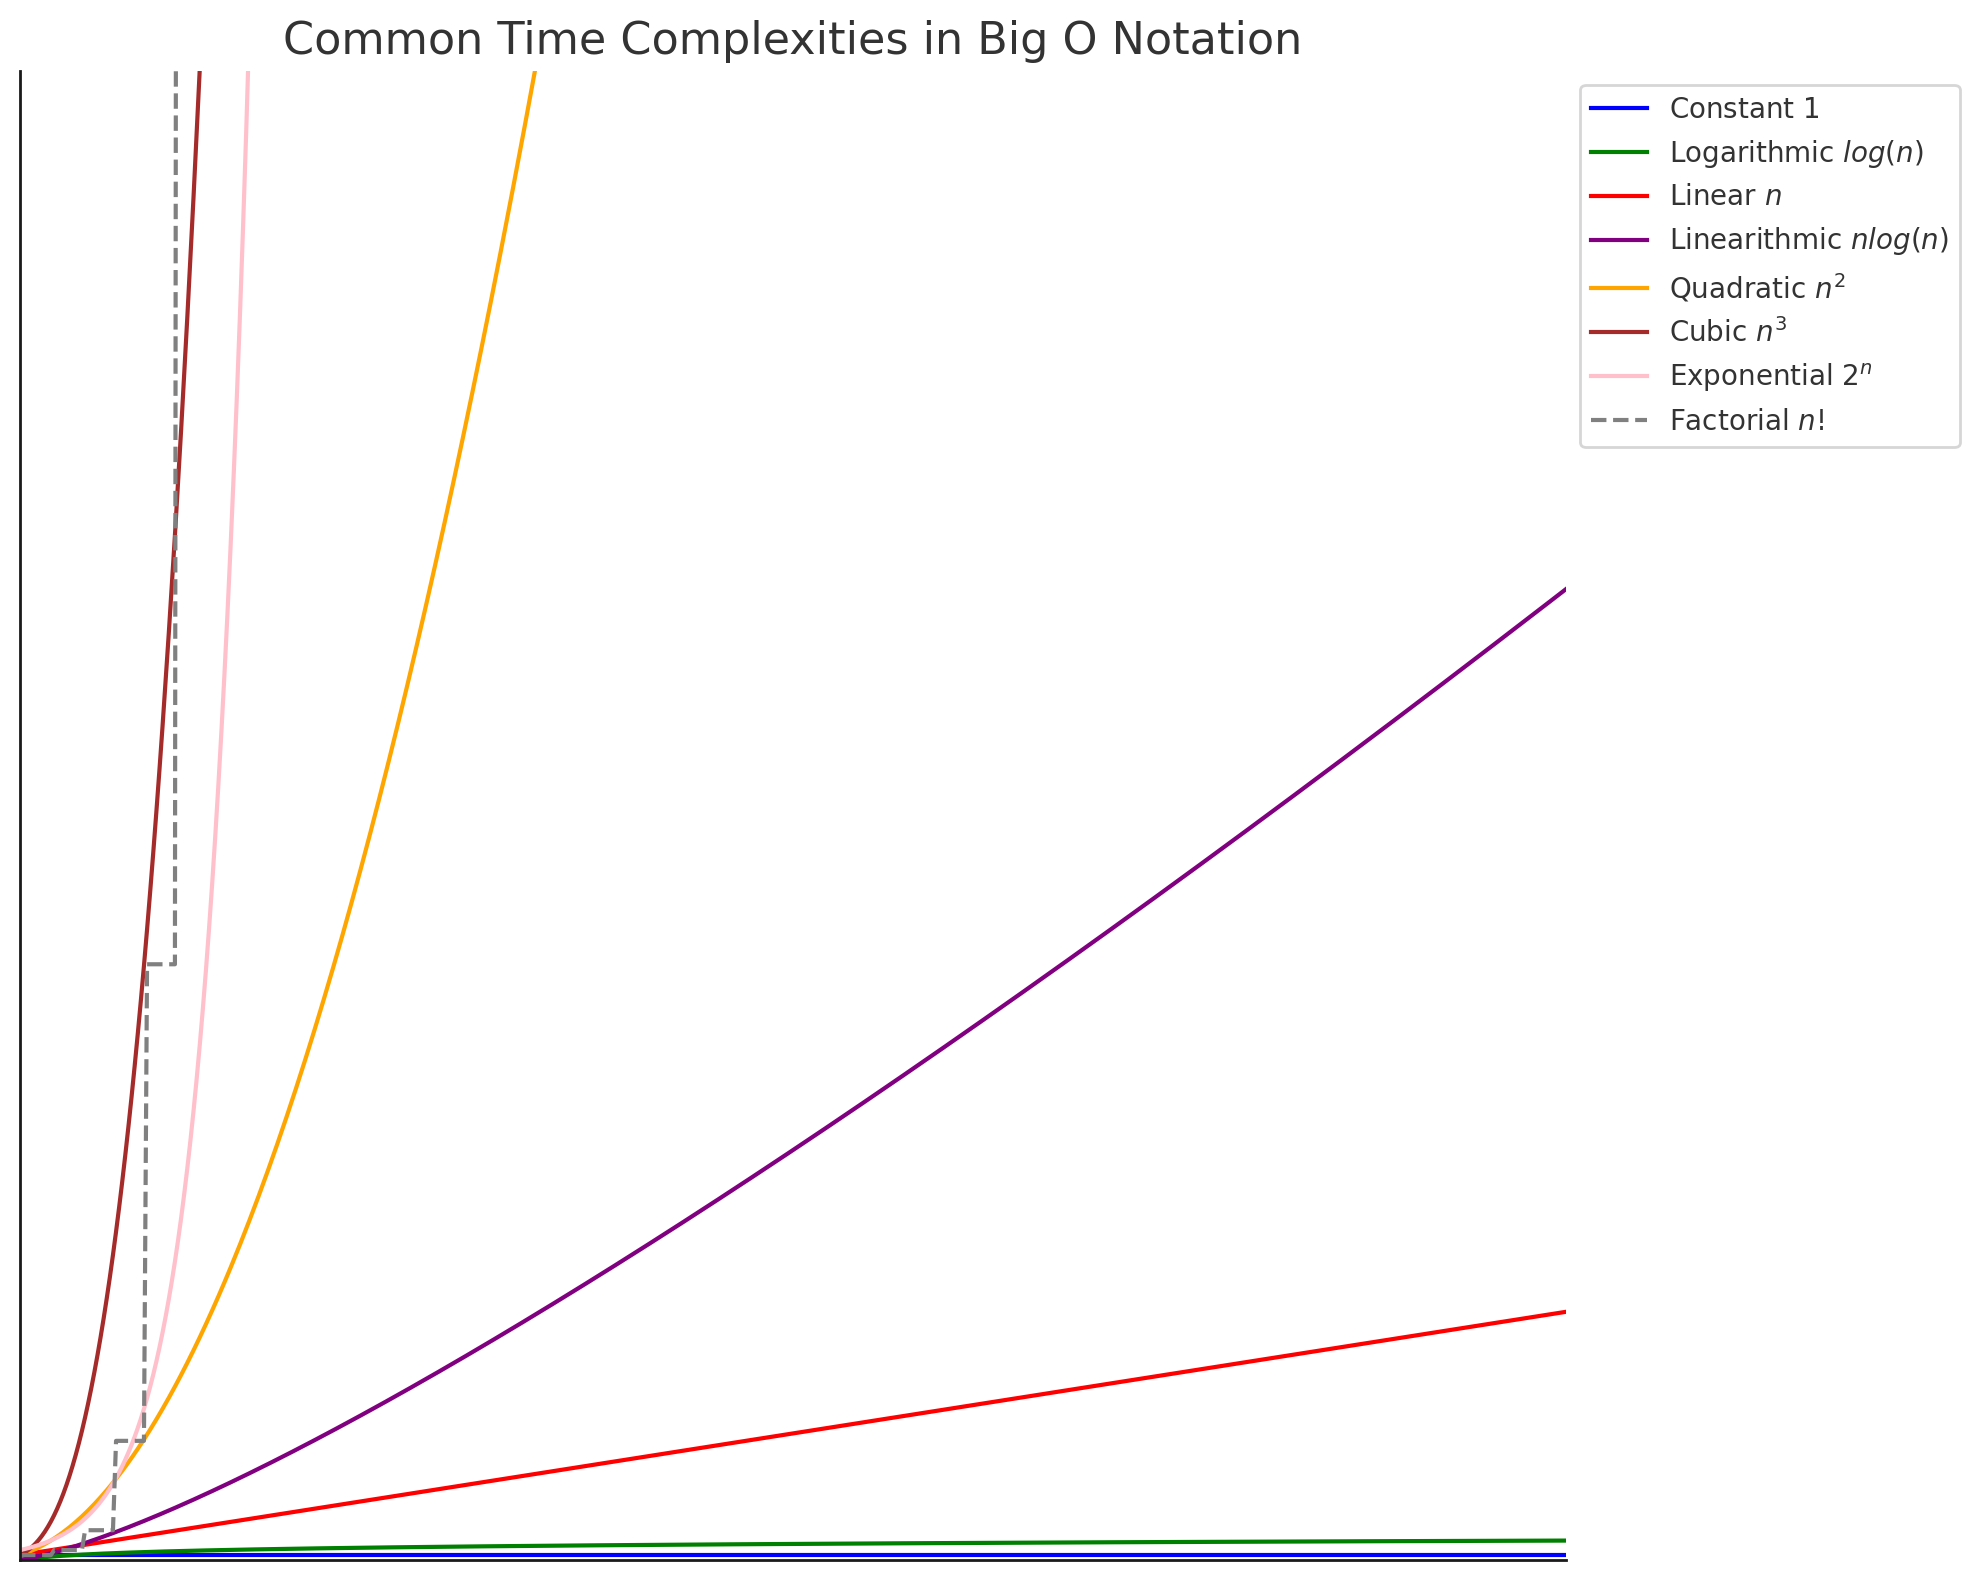
\includegraphics[width=0.8\linewidth]{Images/time complexity.png}
    \caption{Time Complexity Visualization}
    
\end{figure}
So which space and time complexity does this algorithm fall in? 
\subsubsection{Time Complexity}
To analyze the time complexity, we usually focus on the termination condition or the number of iteration for the algorithm. For the real number $B$ in RPM, each time it is divided by 2 until $B = 1$. Therefore, the total number of iteration will be $\log_2 B$, which is categorized in \( O(\log n) \).
\begin{remark}
    Actually, the time complexity of an algorithm could be shown by strict proof using MI. Here is the proof on the time complexity of RPM.
    \begin{proof}
        We will use mathematical induction to prove that the number of steps in the algorithm is proportional to \( \log_2(B) \).

\noindent \textbf{Base Case:}\\
When \( B = 1 \), the algorithm requires only one step. This is consistent with \( \log_2(1) = 0 \), which satisfies our complexity class \( O(\log n) \).

\noindent \textbf{Inductive Hypothesis:}\\
Assume that for a positive integer \( k \), when \( B = k \), the algorithm operates within \( \log_2(k) \) steps.

\noindent \textbf{Inductive Step:}\\
Consider \( B = 2k \). In the first step of the algorithm, \( B \) is halved to \( k \), and \( S \) is doubled. From this point, based on our inductive hypothesis, reaching \( B = 1 \) requires \( \log_2(k) \) steps.

Hence, for \( A = 2k \), the total number of steps is \( \log_2(k) + 1 \). Using the properties of logarithms, we have:
\begin{align*}
\log_2(k) + 1 &= \log_2(k) + \log_2(2) \\
&= \log_2(2k)
\end{align*}

Therefore, for any \( A = 2k \), the total number of steps is also \( \log_2(2k) \), proving that for any positive integer \( A \), the time complexity of the Russian Peasant Multiplication is \( O(\log A) \).
    \end{proof}
\end{remark}
%------------------------------------------------
\subsubsection{Space Complexity}
The space complexity of the Russian Peasant Multiplication algorithm is determined by the amount of memory required to store the operands and the intermediate results. Initially, only two numbers need to be stored: the multiplicands. As the algorithm proceeds, we need additional space to keep track of the current product. Since the algorithm does not use any complex data structures and only requires a fixed number of variables, the space complexity is \( O(1) \), indicating constant space usage. It does not depend on the size of the input operands, as the memory required does not increase with larger numbers.
%------------------------------------------------
\subsection{Exercises}
\begin{exercise}
    A non-recursive Square and Multiply Algorithm to calculate \( b^n \).

\textbf{Precondition:} \( n \) is a positive integer and \( b \) is of any type that can be multiplied.

\textbf{Postcondition:} the value returned is equal \( (b)^n \).

\begin{enumerate}
    \item Show that the algorithm terminates. Let \( a_k \) denote the value of \( a \) after the \( k \)th iteration of the while-loop, and let \( s = \lfloor \lg(n) \rfloor \). Prove by Mathematical Induction on \( k \) that For any nonnegative integer \( k \), after \( k \) iterations of the while-loop:
    $$2^{s-k} \le a_k < 2^{s-k+1}$$
    \item  Proof of correctness. Use Mathematical Induction on \( k \) to prove For any nonnegative integer \( k \), after \( k \) iterations of the while-loop:
\[ (\text{square})^a \times \text{product} = (b)^n \]
\end{enumerate}
\end{exercise}
\begin{algorithm}
    \caption{Square and Multiply Algorithm}
    \begin{algorithmic}[1]
    \State $product \gets 1$
    \State $square \gets b$
    \State $a \gets n$
    \While{$a > 1$}
        \If{$a \mod 2 \neq 0$} \Comment{If $a$ is odd}
            \State $product \gets product \times square$
        \EndIf
        \State $square \gets square \times square$
        \State $a \gets \lfloor a / 2 \rfloor$ \Comment{Integer division}
    \EndWhile
    \State \Return $product \times square$
    \end{algorithmic}
\end{algorithm}
\begin{proof}[1]
    \textit{Base Case} \(k=0\):
For \(k = 0\), \(a_0 = n\), which is the initial value of \(a\). Since \(s = \left\lfloor \lg(n) \right\rfloor\), it is the greatest integer less than or equal to \(\lg(n)\), therefore \(2^s \leq n < 2^{s+1}\). So, for \(k = 0\), the predicate holds because:
\[
\frac{2^s}{2^0} \leq a_0 = n < 2 \times \frac{2^s}{2^0}
\]

\textit{Inductive Step}:
Assume \(P(k)\) holds for some nonnegative integer \(k\). That is:
\[
\frac{2^s}{2^k} \leq a_k < 2 \times \frac{2^s}{2^k}
\]
We need to show \(P(k+1)\) holds. During each iteration, \(a\) is halved (integer division by 2), which gives us:
\[
a_{k+1} = \left\lfloor \frac{a_k}{2} \right\rfloor
\]

Since \(a_k\) is an integer, \(\left\lfloor \frac{a_k}{2} \right\rfloor\) will either be \(\frac{a_k}{2}\) or \(\frac{a_k - 1}{2}\), depending on whether \(a_k\) is even or odd. Thus, we have:
\[
\frac{2^s}{2^{k+1}} \leq \left\lfloor \frac{a_k}{2} \right\rfloor < 2 \times \frac{2^s}{2^{k+1}}
\]

Since \(a_k < 2 \times \frac{2^s}{2^k}\), dividing by 2 gives \(\frac{a_k}{2} < \frac{2^s}{2^k}\), and therefore:
\[
a_{k+1} < 2 \times \frac{2^s}{2^{k+1}}
\]

Similarly, \(\frac{2^s}{2^k} \leq a_k\) implies \(\frac{2^s}{2^{k+1}} \leq \frac{a_k}{2}\), so we have:
\[
\frac{2^s}{2^{k+1}} \leq a_{k+1}
\]
This completes the inductive step and thus, by induction, \(P(k)\) holds for all nonnegative integers \(k\).
\end{proof}
\begin{proof}[2]
    We need to prove that after \(k\) iterations of the while-loop, the invariant holds:
\[
(\text{square})^a \times \text{product} = b^n
\]

\textit{Base Case} \(k=0\):
Initially, \(\text{product} = 1\), \(\text{square} = b\), and \(a = n\). So,
\[
(\text{square})^a \times \text{product} = b^n
\]
is trivially true.

\textit{Inductive Step}:
Assume the invariant holds after \(k\) iterations, i.e.,
\[
(\text{square}_k)^{a_k} \times \text{product}_k = b^n
\]
Now, consider the \(k+1\)th iteration. There are two cases:

\textit{Case 1} (\(a_k\) is odd):
The product is updated by multiplying it with \(\text{square}_k\), and we have:
\[
\text{product}_{k+1} = \text{product}_k \times \text{square}_k
\]
Since \(a_k\) is odd, we can write \(a_k = 2m + 1\) for some integer \(m\), and after the iteration, \(a\) becomes \(a_{k+1} = m\). The invariant becomes:
\[
(\text{square}_k)^{2m+1} \times \text{product}_k = (\text{square}_k)^m \times \text{product}_{k+1} = b^n
\]

\textit{Case 2} (\(a_k\) is even):
The product remains the same, and \(a_k\) can be written as \(2m\), so the invariant remains:
\[
(\text{square}_k)^{2m} \times \text{product}_k = (\text{square}_k)^m \times \text{product}_k = b^n
\]
since \(\text{square}_{k+1} = (\text{square}_k)^2\) and \(a_{k+1} = m\).

In both cases, after the iteration, \(\text{square}\) is squared, so we get:
\[
\text{square}_{k+1} = (\text{square}_k)^2
\]
and therefore, the invariant still holds as:
\[
(\text{square}_{k+1})^{a_{k+1}} \times \text{product}_{k+1} = b^n
\]

Thus, by mathematical induction, the invariant holds true for every iteration of the loop, proving the correctness of the algorithm.
\end{proof}

